% to run: lualatex ttZ_EFT.tex
\RequirePackage{luatex85}
\documentclass[tikz, border=10pt]{standalone}

\usepackage[compat=1.1.0]{tikz-feynman}

\newcommand{\Ptop}{\ensuremath{\mathrm{t}}}
\newcommand{\Pg}{\ensuremath{\mathrm{g}}}
\newcommand{\Pq}{\ensuremath{\mathrm{q}}}
\newcommand{\PH}{\ensuremath{\mathrm{H}}}
\newcommand{\PW}{\ensuremath{\mathrm{W}}}

\makeatletter
\tikzset{
  position/.style args={#1 degrees from #2}{
    at=(#2.#1), anchor=#1+180, shift=(#1:\tikz@node@distance)
  }
}
\makeatother

\begin{document}
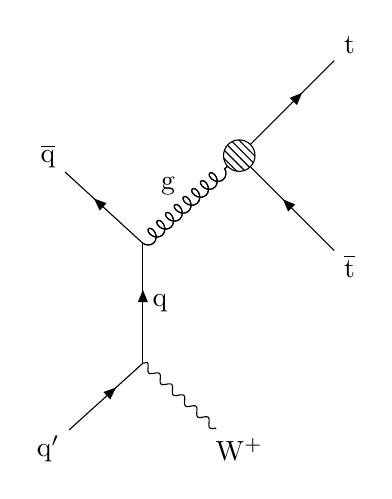
\begin{tikzpicture}
  \begin{feynman}
    \diagram [arrow size=1pt, vertical=a to b] {
      i1 [particle=\(\overline \Pq\)] -- [anti fermion] a -- [gluon] c [blob, minimum size=0.4cm],
      a -- [anti fermion, edge label=\(\Pq\)] b,
      f1 [particle=\(\PW^+\)] -- [boson] b -- [anti fermion] f2 [particle=\(\Pq^\prime\)],
    };

    \vertex [position=45 degrees from c] (d) {\(\Ptop\)};
    \vertex [position=-45 degrees from c] (e) {\(\overline \Ptop\)};

    \diagram* [arrow size=1pt] {
      (a) -- [gluon, edge label=\(\Pg\)] (c),
      (d) -- [anti fermion] (c) -- [anti fermion] (e);
    };
  \end{feynman}
\end{tikzpicture}
\end{document}
